\documentclass[a4paper,12pt,dvipsnames]{letter}
%
\usepackage[a4paper]{geometry}
\usepackage[utf8]{inputenc}
\usepackage[T1]{fontenc}
\usepackage{lmodern}
\usepackage{xcolor}
\usepackage{colortbl}
\usepackage{multirow}
\usepackage{courier}
\usepackage{array}
\usepackage{booktabs}
\usepackage{amsmath} 
\usepackage{amsfonts} 
\usepackage{amssymb}
\usepackage{wasysym}
\usepackage{marvosym}
\usepackage{stmaryrd}
\usepackage{tikz}
\usepackage{textcomp}
\usepackage{enumitem}
\usepackage{graphicx}
%
% set page geometry
\geometry{top=0.5cm,left=1cm,right=4cm,bottom=1cm}
\pagestyle{empty}
%
% special columns
\newcolumntype{L}[1]{>{\raggedright\let\newline\\\arraybackslash\hspace{0pt}}m{#1}}
\newcolumntype{C}[1]{>{\centering\let\newline\\\arraybackslash\hspace{0pt}}m{#1}}
\newcolumntype{R}[1]{>{\raggedleft\let\newline\\\arraybackslash\hspace{0pt}}m{#1}}
%
% increase row height
\renewcommand{\arraystretch}{1.0}
%
\makeatletter
\newcommand{\thickhline}{\noalign {\ifnum 0=`}\fi \hrule height 2pt \futurelet \reserved@a \@xhline}
\newcommand{\medhline}{\noalign {\ifnum 0=`}\fi \hrule height 1pt \futurelet \reserved@a \@xhline}
\newcolumntype{"}{@{\hskip\tabcolsep\vrule width 1pt\hskip\tabcolsep}}
\makeatother
%
\newlength{\Oldarrayrulewidth}
\newcommand{\Cline}[2]{\noalign{\global\setlength{\Oldarrayrulewidth}{\arrayrulewidth}}\noalign{\global\setlength{\arrayrulewidth}{#1}}\cline{#2}\noalign{\global\setlength{\arrayrulewidth}{\Oldarrayrulewidth}}}
%
% my commands
\newcommand{\rot}[1]{\textcolor{red}{#1}}
\newcommand{\blau}[1]{\textcolor{blue}{#1}}
\newcommand{\grun}[1]{\textcolor{Green}{#1}}
\newcommand{\gelb}[1]{\textcolor{Yellow}{#1}}
\newcommand{\rotb}[1]{\textcolor{red}  {\textbf{#1}}}
\newcommand{\grnb}[1]{\textcolor{Green}{\textbf{#1}}}
\newcommand{\blub}[1]{\textcolor{blue} {\textbf{#1}}}
\newcommand{\oranb}[1]{\textcolor{BurntOrange} {\textbf{#1}}}
\newcommand{\gelbb}[1]{\textcolor{Yellow} {\textbf{#1}}}
\newcommand{\radio}[1]{\textcolor{blue}{#1}}
\newcommand{\call}[1]{\textcolor{blue}{{#1}}}
\newcommand{\button}[1]{\textbf{#1}}
\newcommand{\degC}{\textdegree{}C}
\newcommand{\Deg}{\textdegree{}}
\newcommand{\ok}[1]{\textcolor{Green}{\textbf{#1}}}
\newcommand{\boat}[1]{\textcolor{Blue}{\textbf{#1}}}
\newcommand{\warn}[1]{\textcolor{Red}{\textbf{#1}}}
\newcommand{\myHead}[1]{{\LARGE\textsc{\textbf{#1}}}}
\newcommand{\myhead}[1]{{\large\textsc{\textbf{#1}}}}
% itemize
\renewcommand{\labelitemi}{{$\bullet$\;}}
\renewcommand{\labelitemii}{{$\bullet$\;}}
\renewcommand{\labelitemiii}{$\bullet$\;}
\renewcommand{\labelitemiv}{$\bullet$\;}
% color bullets
\newcommand{\bi}{\textcolor{ProcessBlue}{$\bullet$\;}}
\newcommand{\ri}{\textcolor{Red}{$\bullet$\;}}
\newcommand{\gi}{\textcolor{Green}{$\bullet$\;}}
\newcommand{\yi}{\textcolor{Yellow}{$\bullet$\;}}
\newcommand{\vi}{\textcolor{Plum}{$\bullet$\;}}
\newcommand{\mi}{\textcolor{Magenta}{$\bullet$\;}}
\newcommand{\oi}{\textcolor{Orange}{$\bullet$\;}}
\newcommand{\ai}{\textcolor{Apricot}{$\bullet$\;}}
\renewcommand{\ni}{\textcolor{Brown}{$\bullet$\;}}
\newcommand{\si}{\textcolor{SpringGreen}{$\bullet$\;}}
%
\newcommand{\mr}[2]{\multirow{#1}{*}{#2}}
\newcommand{\mcl}[2]{\multicolumn{#1}{|c|}{#2}}
\newcommand{\tb}[1]{\textbf{#1}}
\newcommand{\tp}[1]{\textsf{#1}}
\renewcommand{\tp}[1]{\fontfamily{cmss}\selectfont #1}
\newcommand{\refn}{Ref.\,\fontfamily{ppl}\selectfont\#\fontfamily{cmss}\selectfont}
%
% some info
\pdfinfo{%
  /Title    (FPP Training)
  /Author   (funkyfranky)
  /Creator  ()
  /Producer ()
  /Subject  ()
  /Keywords (F/A-18C, Hornet, Kneeboard, Procedures)
}
%
% Note: max 29 items per page
\begin{document}
\texttt{
% SCRAMBLE START (Extended)
\begin{itemize}
 \item[] \myHead{Radio Comms}
 %
 \vspace{1em}
 \item[] \myhead{CVN-74 USS Stennis}
 \item[\bi] Marshal 305\,MHz
 \item[\bi] LSO 264\,MHz
 \item[\bi] Tower 127.5\,MHz
 \item[\bi] TACAN 74X
 \item[\bi] ICLS Ch\,1
 %
 \vspace{1em}
 \item[] \myhead{AWACS}
 \item[\bi] E-2D Wizard (overhead Stennis)
 \begin{itemize}
  \item[\gi] 260\,MHz
 \end{itemize}
 \item[\gi] E-3D Magic (near Batumi)
 \begin{itemize}
  \item[\gi] 260\,MHz
 \end{itemize}
 %
 \vspace{1em}
 \item[] \myhead{Tanker}
 \item[\bi] S-3B Texaco (overhead Stennis)
 \begin{itemize}
  \item[\gi] 250\,MHz
  \item[\gi] TACAN 1Y
 \end{itemize}
 \item[\bi] KC-135 Arco (near Batumi)
 \begin{itemize}
  \item[\bi] 260\,MHz
  \item[\bi] TACAN 3Y
 \end{itemize} 
\end{itemize}
% ---------------------------------------------------------------------------------------------------
\newpage
% PRE-FLIGHT
\begin{itemize}
 \item[] \myHead{Bombing Range Kobuleti X}
 \item[\ri] Target: Unarmed Fuel Truck
 \item[\ri] Position: N042\,11\;22 E42\,11\,22
\end{itemize}
\begin{center}
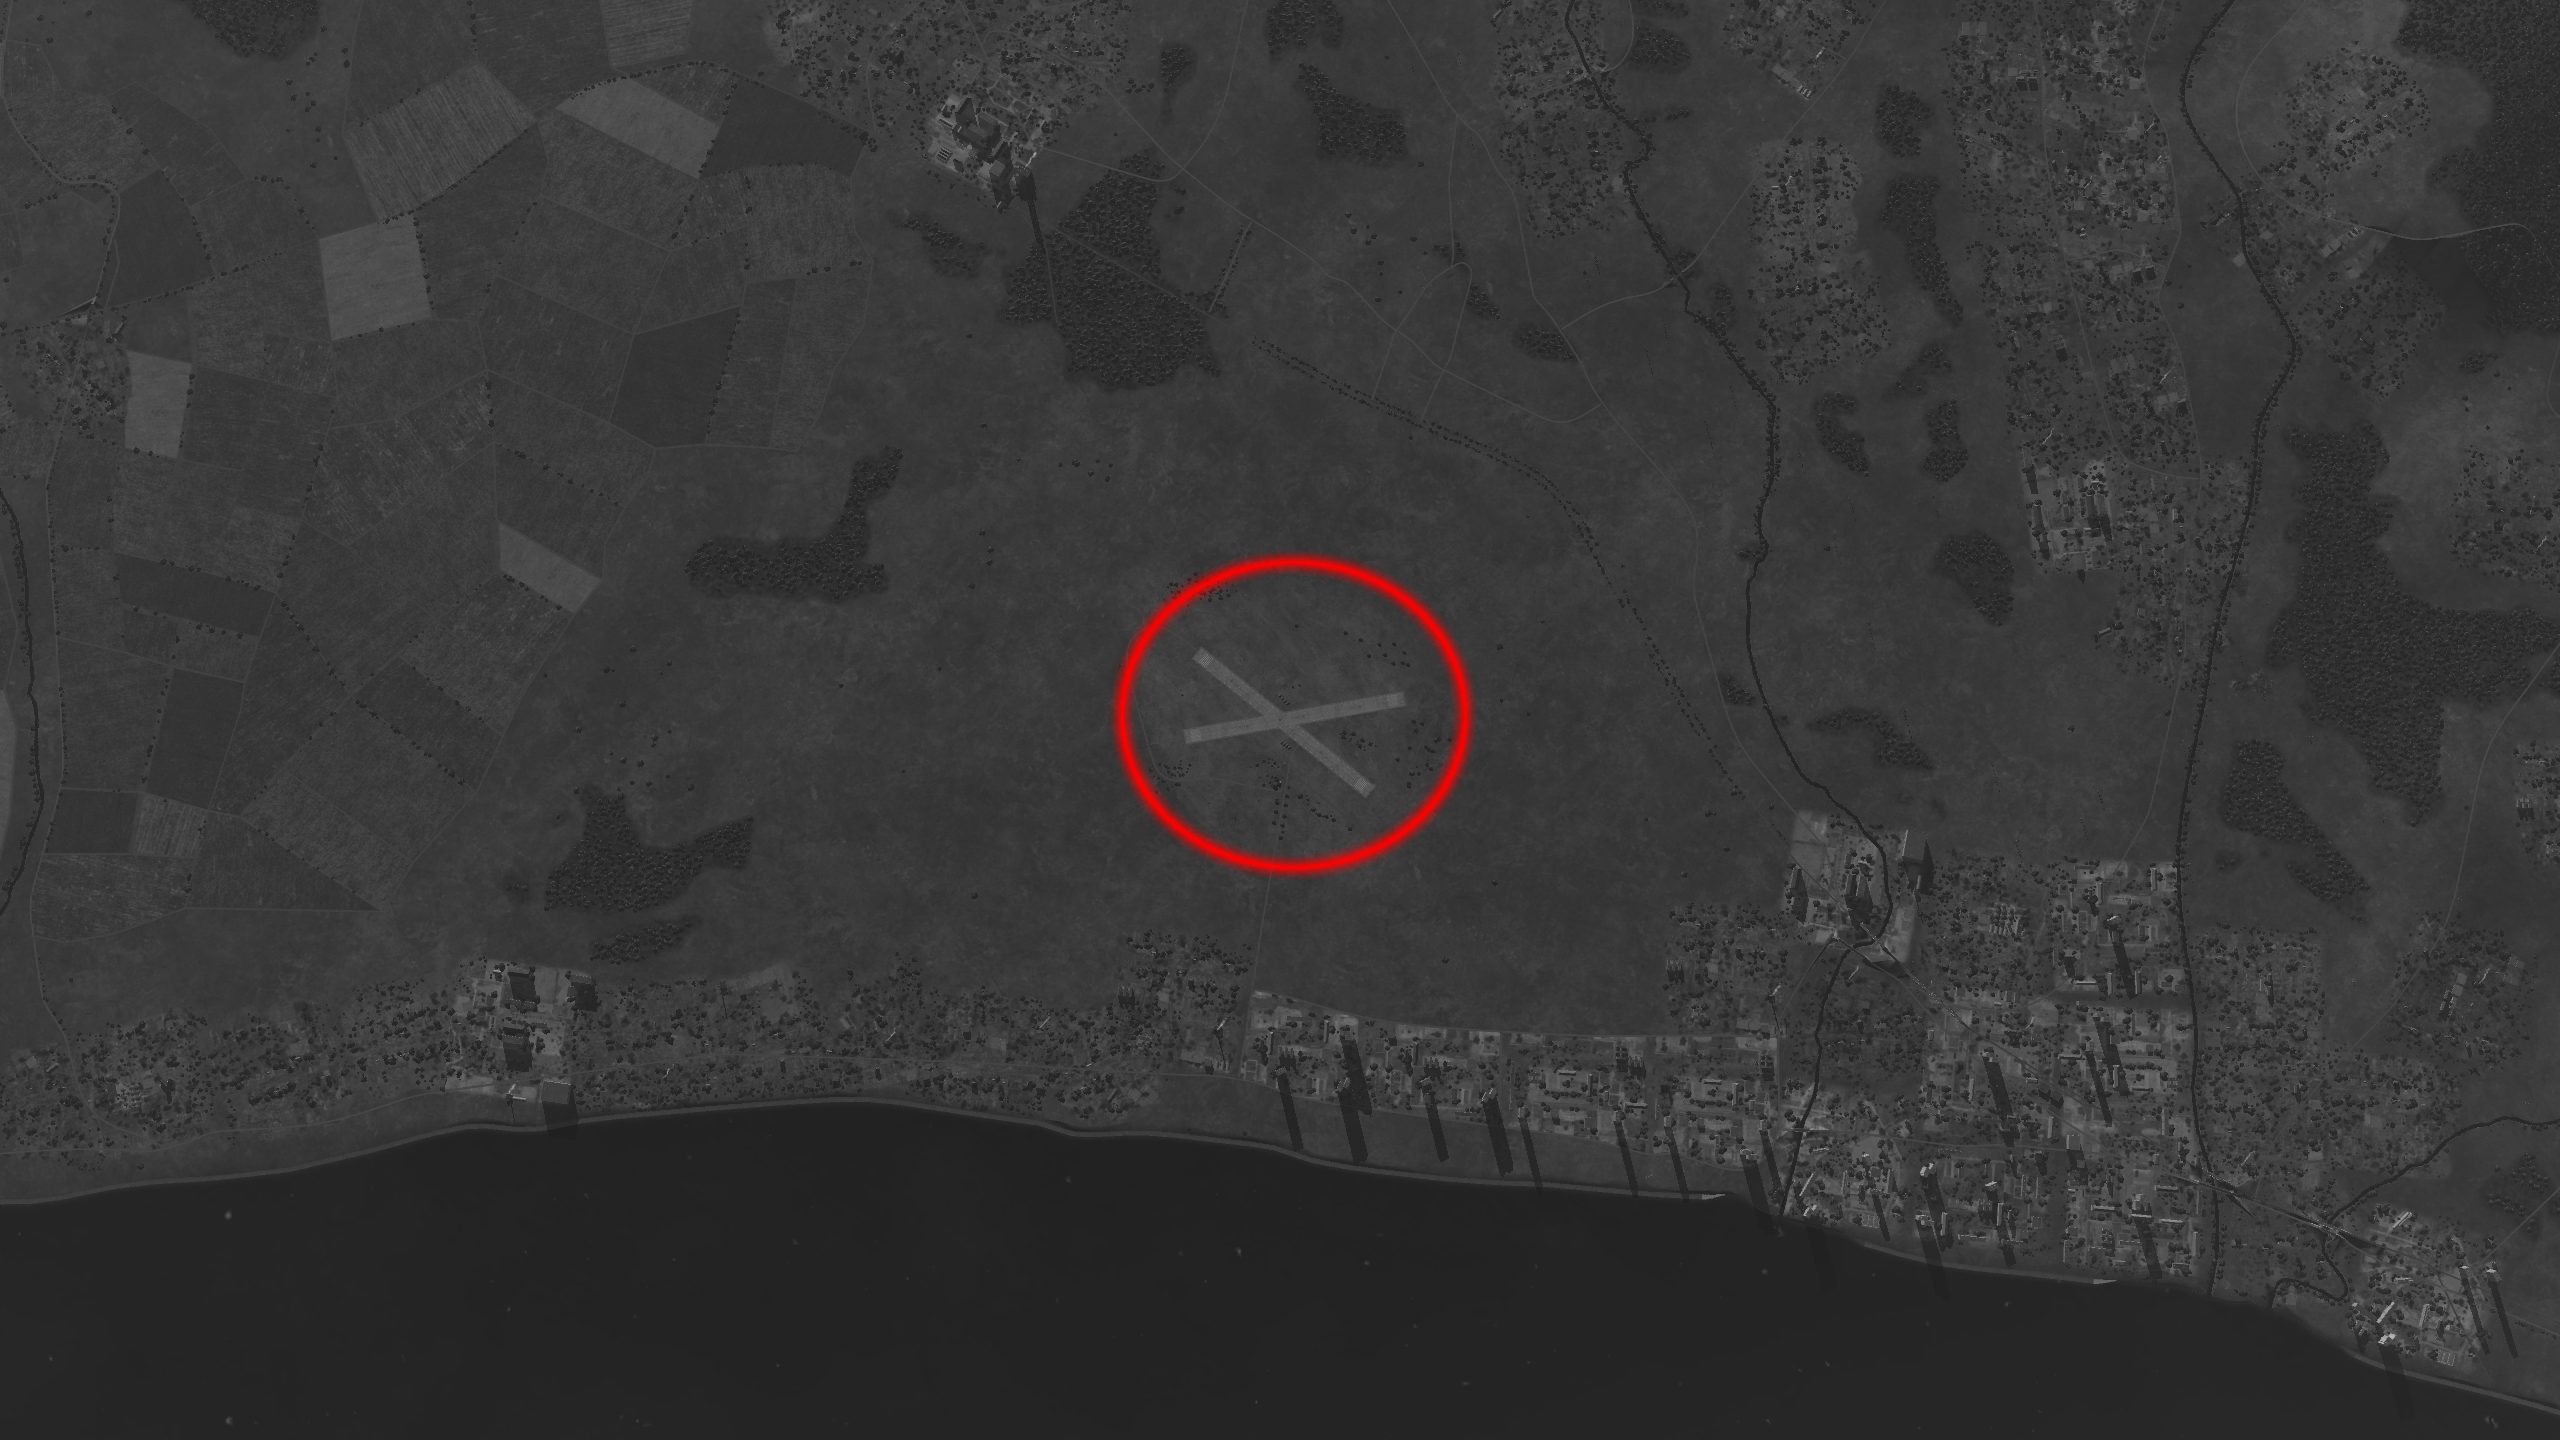
\includegraphics[width=0.7\linewidth]{../gimp/Range_Kobuleti_Sat.png}
\end{center}
%
% ---------------------------------------------------------------------------------------------------
\newpage
% PRE-FLIGHT
\begin{itemize}
 \item[] \myHead{Bombing Range Kutaisi}
 \item[\ri] Target: Unarmed Vehicles (moving)
 \item[\ri] Position: unknown
 \item[\ri] Target: Tech Combine
 \item[\ri] Position: N042\,11\;22 E42\,11\,22 
\end{itemize}
\begin{center}
 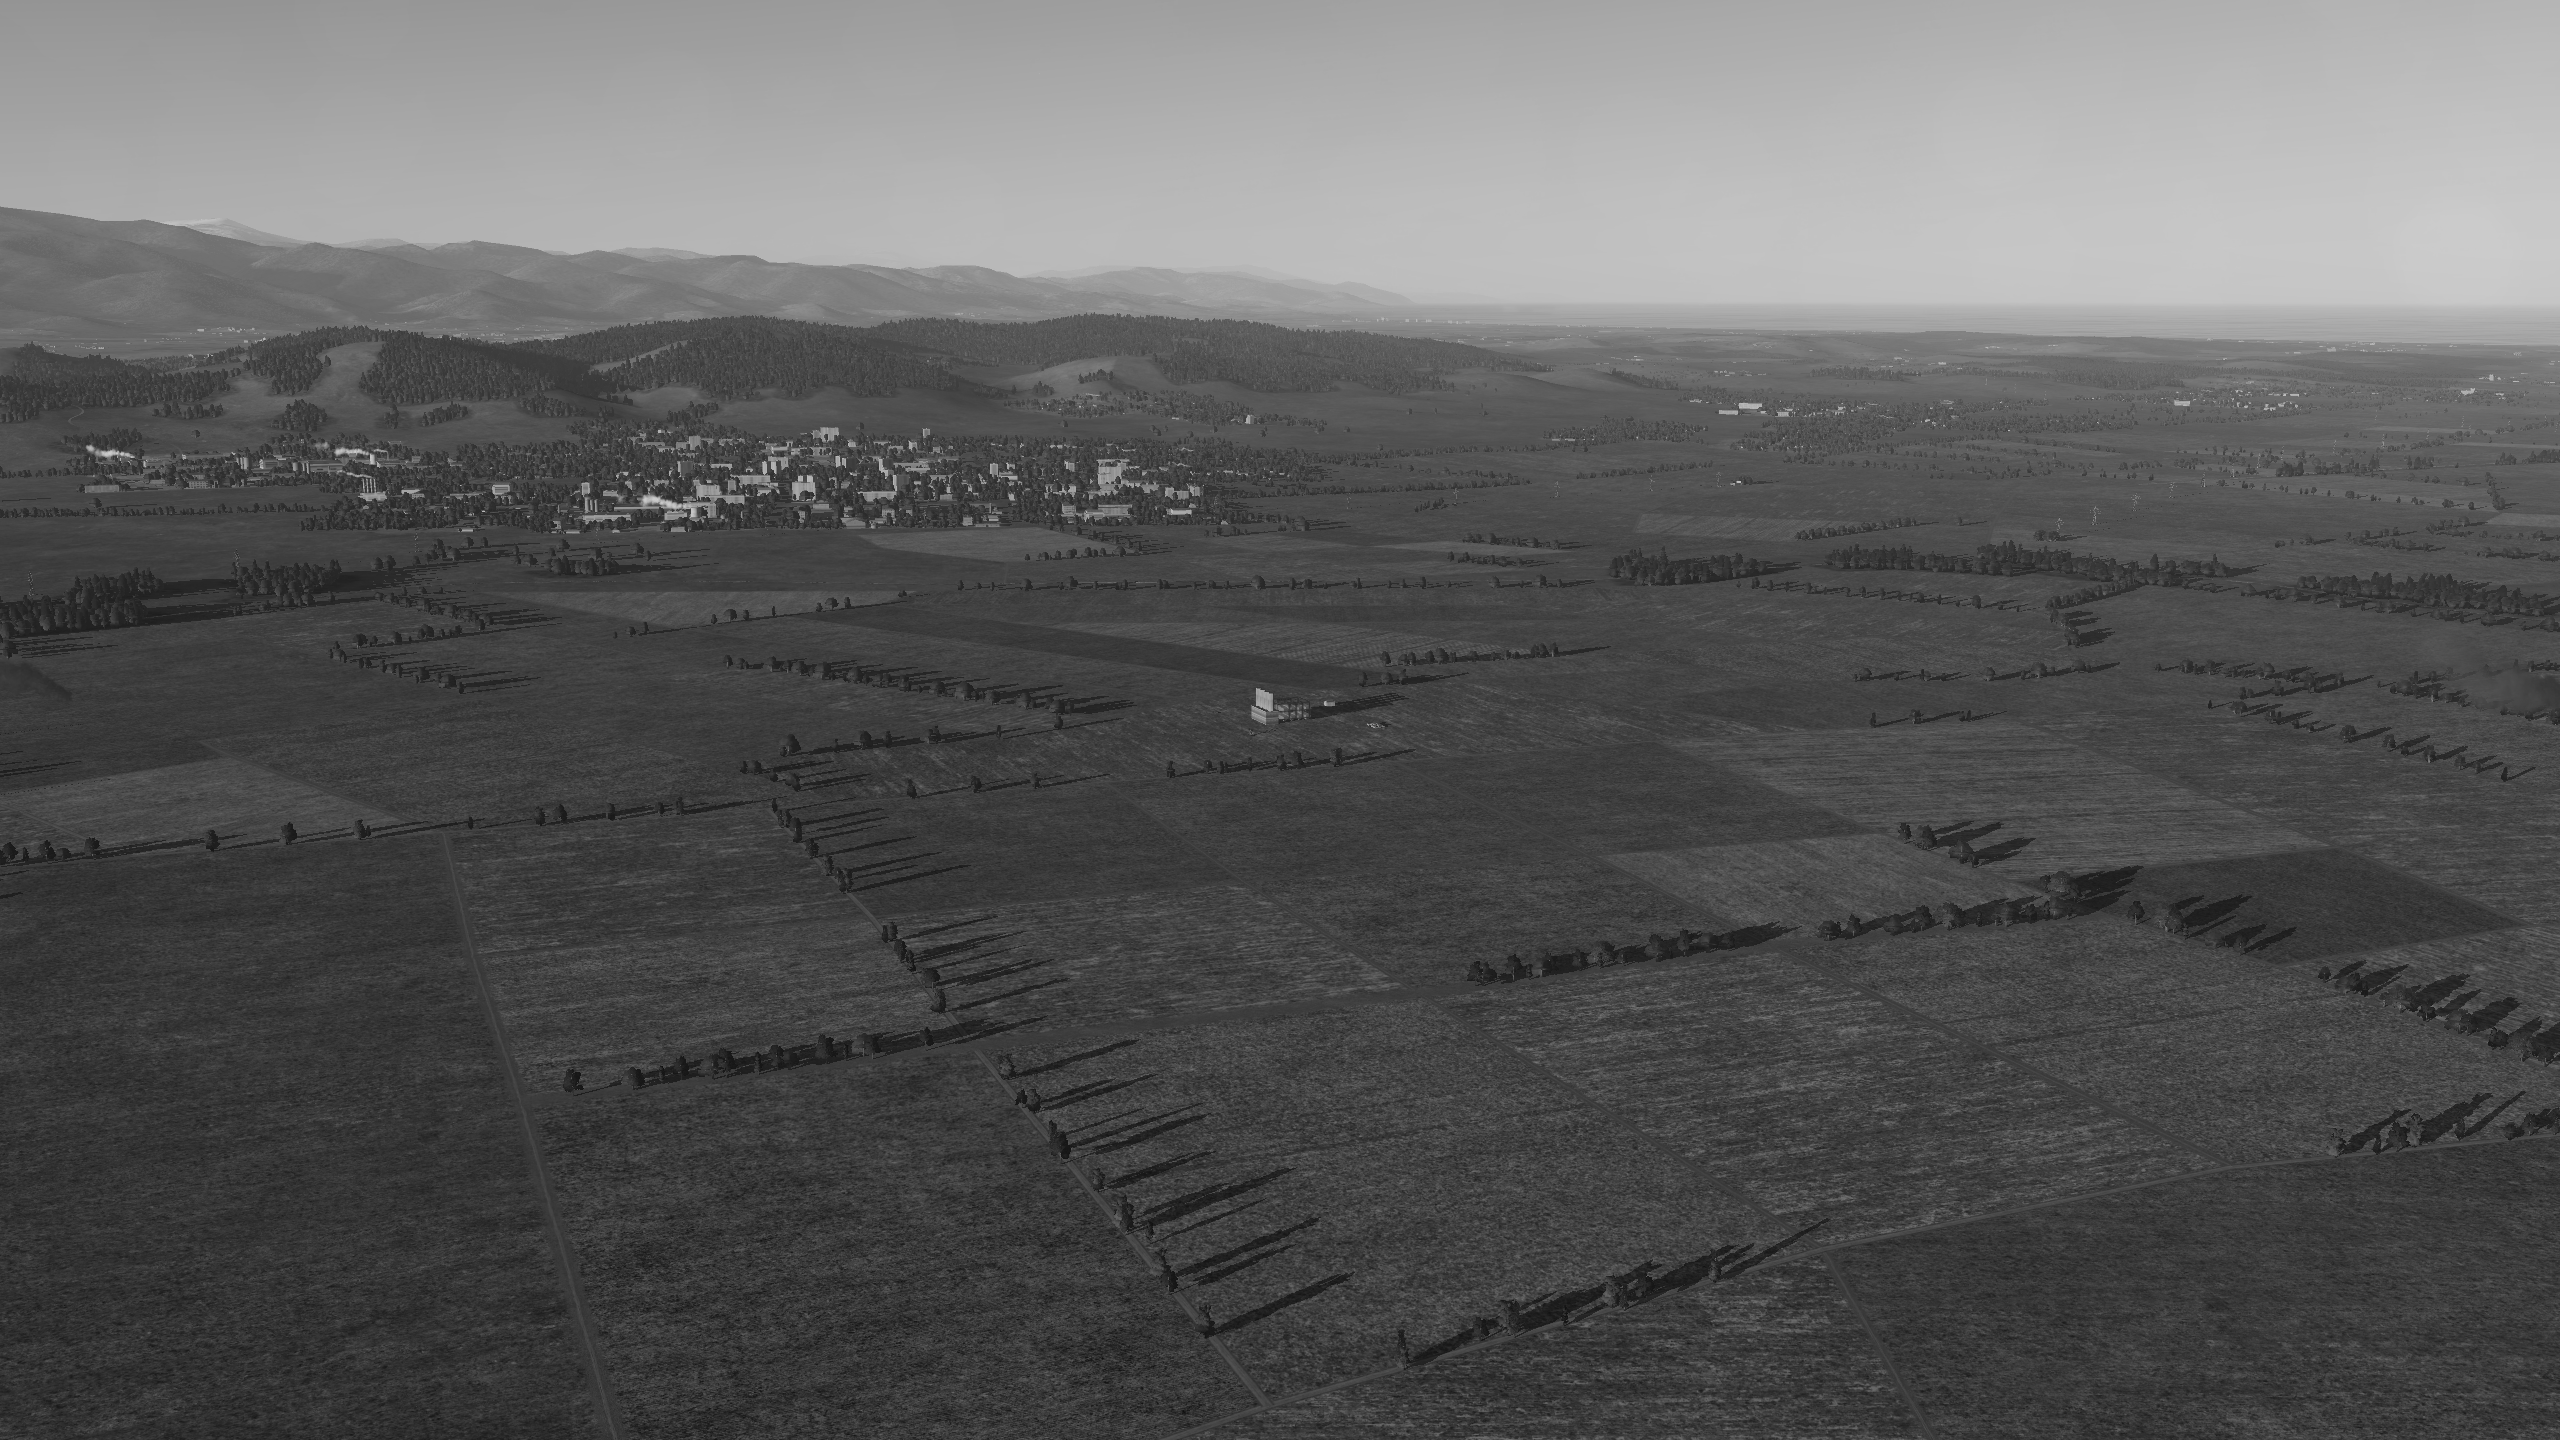
\includegraphics[width=0.7\linewidth]{../gimp/Range_Kutaisi_Pic1.png}
\end{center}
%
% ---------------------------------------------------------------------------------------------------
\newpage
% PRE-FLIGHT
\begin{itemize}
 \item[] \myHead{Air-to-Air: Easy}
 \item[\ri] Target: MiG-19 and MiG-21 drones
 \item[\ri] Position: Near Maykop
\end{itemize}
%
% ---------------------------------------------------------------------------------------------------
\newpage
% PRE-FLIGHT
\begin{itemize}
 \item[] \myHead{Air-to-Air: Hard}
 \item[\ri] Target: Su-27
 \item[\ri] Position: Near Maykop
 \item[\ri] Target: MiG-31
 \item[\ri] Position: Near XYZ
\end{itemize}
%
% ---------------------------------------------------------------------------------------------------
\newpage
% PRE-FLIGHT
\begin{itemize}
 \item[] \myHead{Air-to-Ground: Hard}
 \item[\ri] Target: FARP Skala
 \item[\ri] Position: N042\,11\;22 E42\,11\,22 
 \item[\ri] Threads: Su-27, MiG-31
 \item[\ri] Threads: ZU-XY, Manpads
\end{itemize}
\begin{center}
 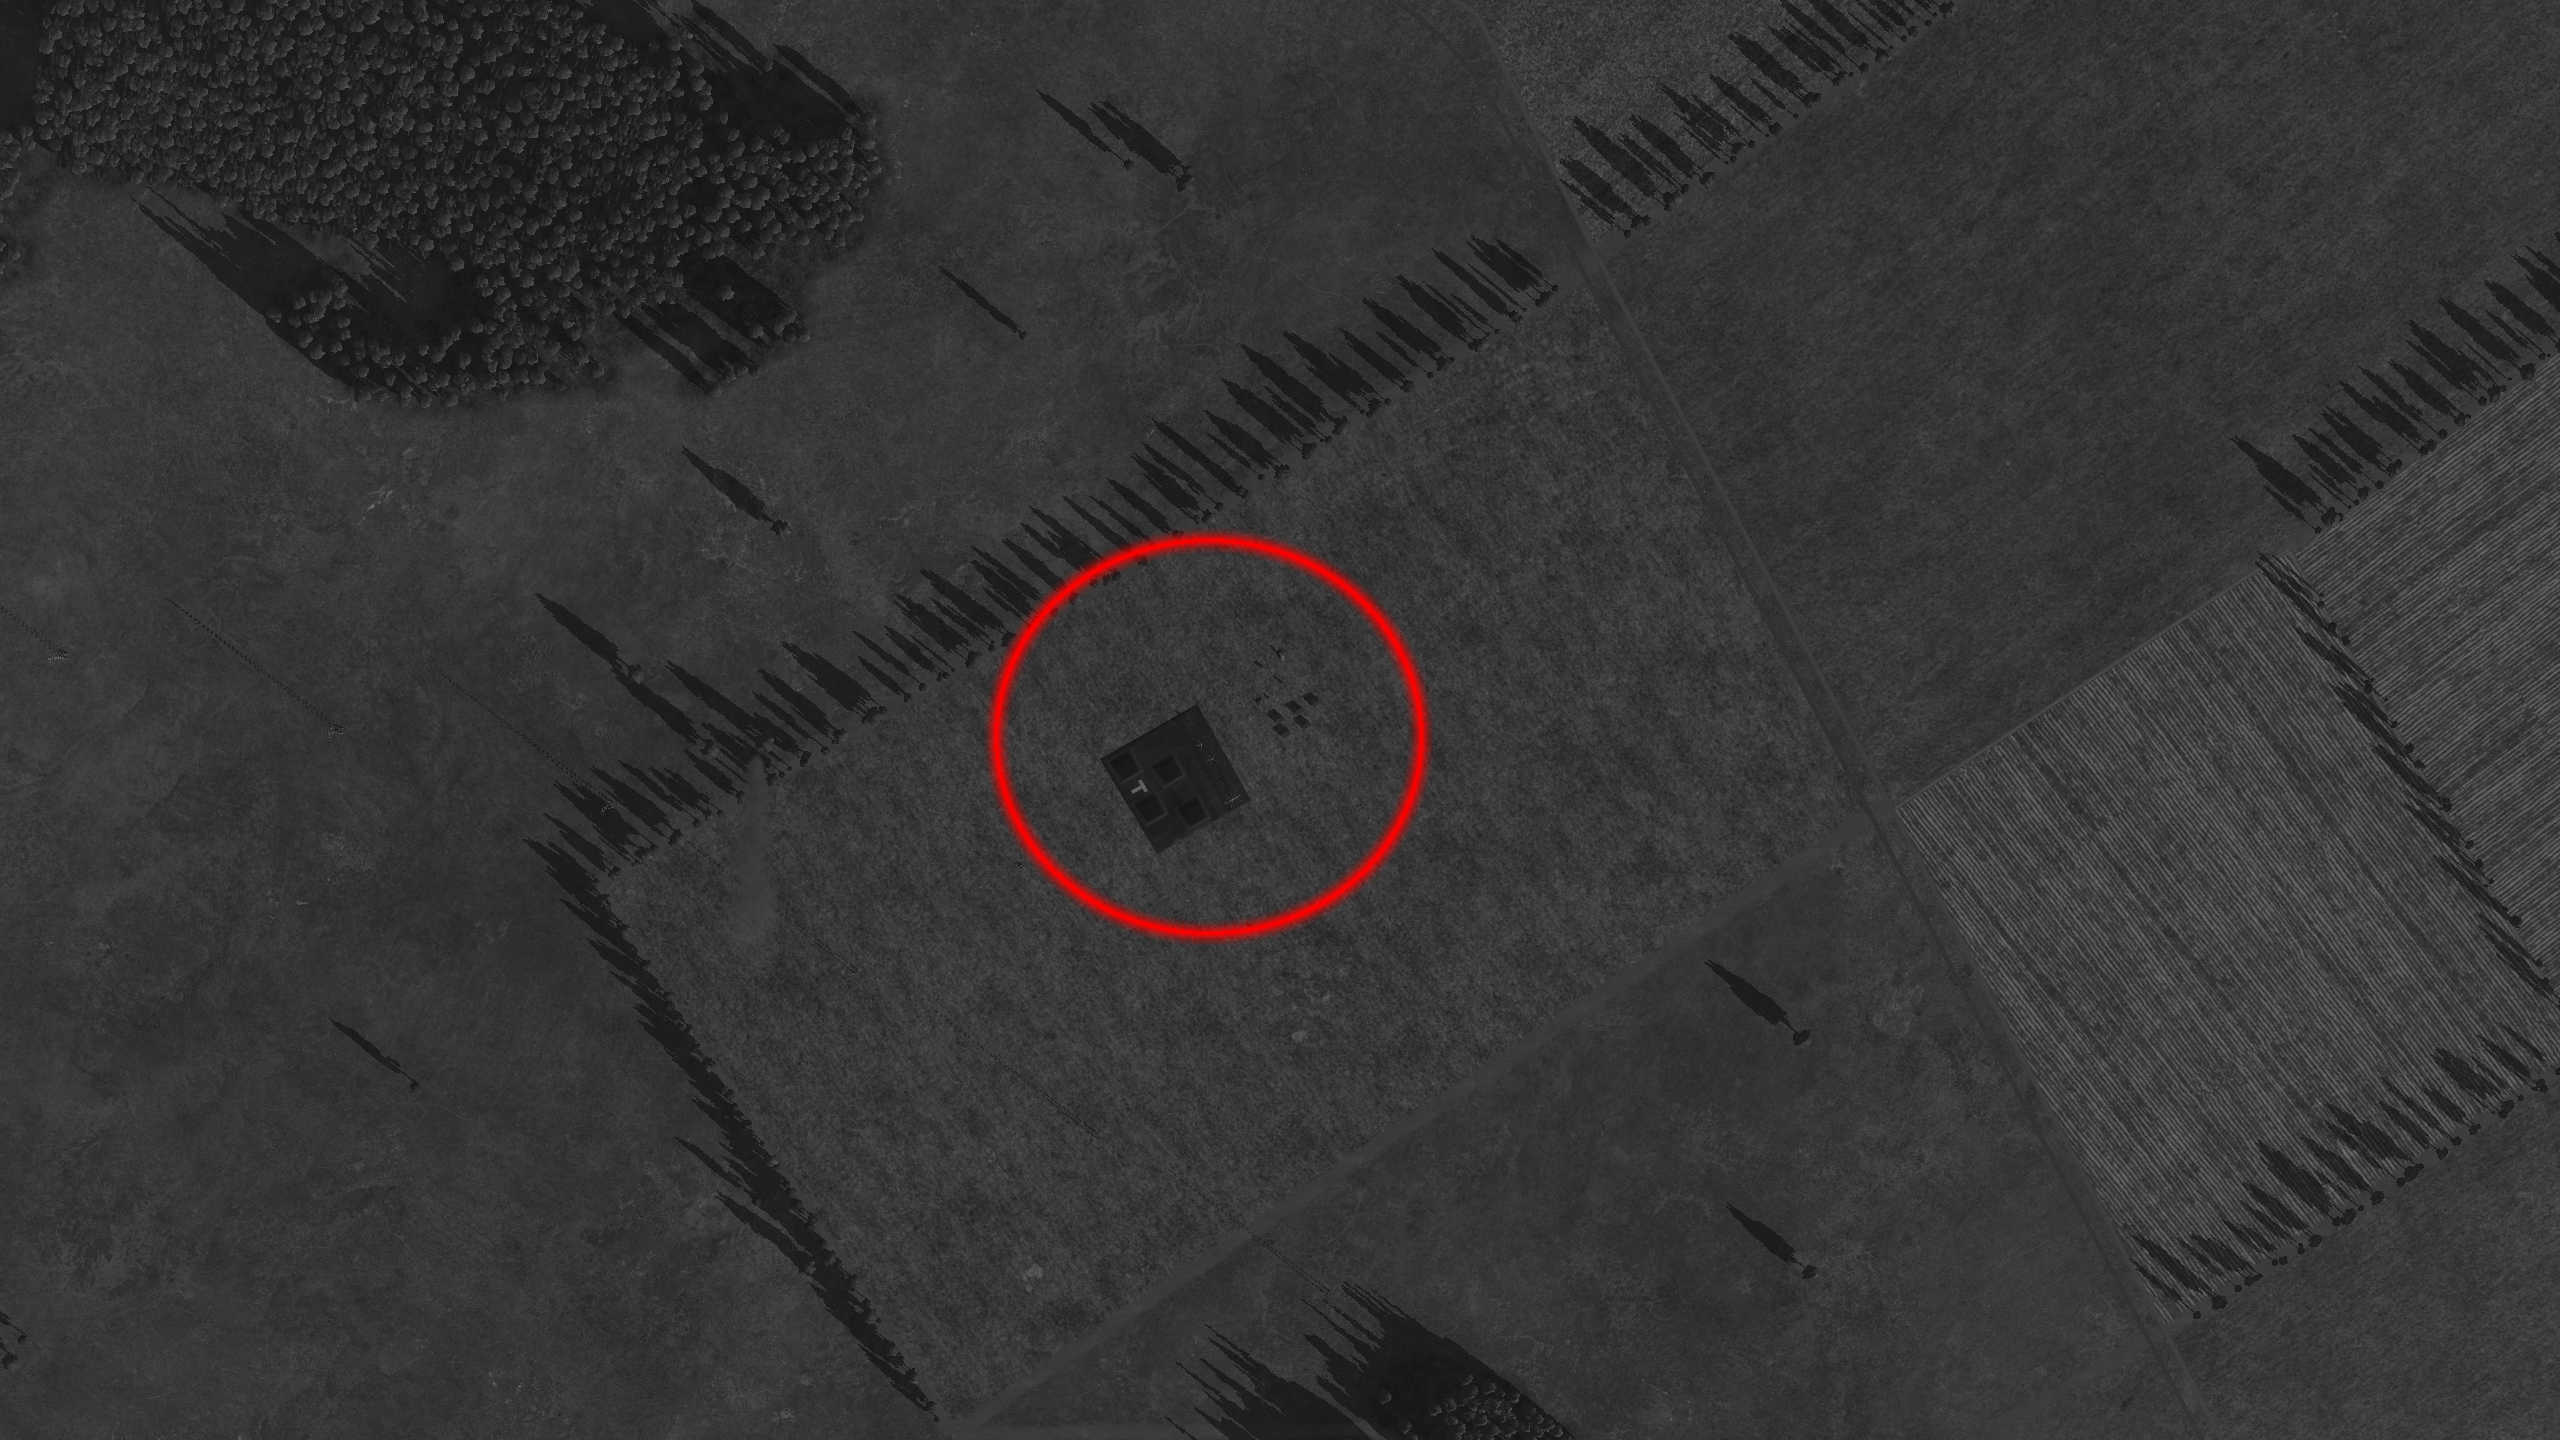
\includegraphics[width=0.7\linewidth]{../gimp/FARP_Skala_Sat.png}
\end{center}
%
\begin{center}
 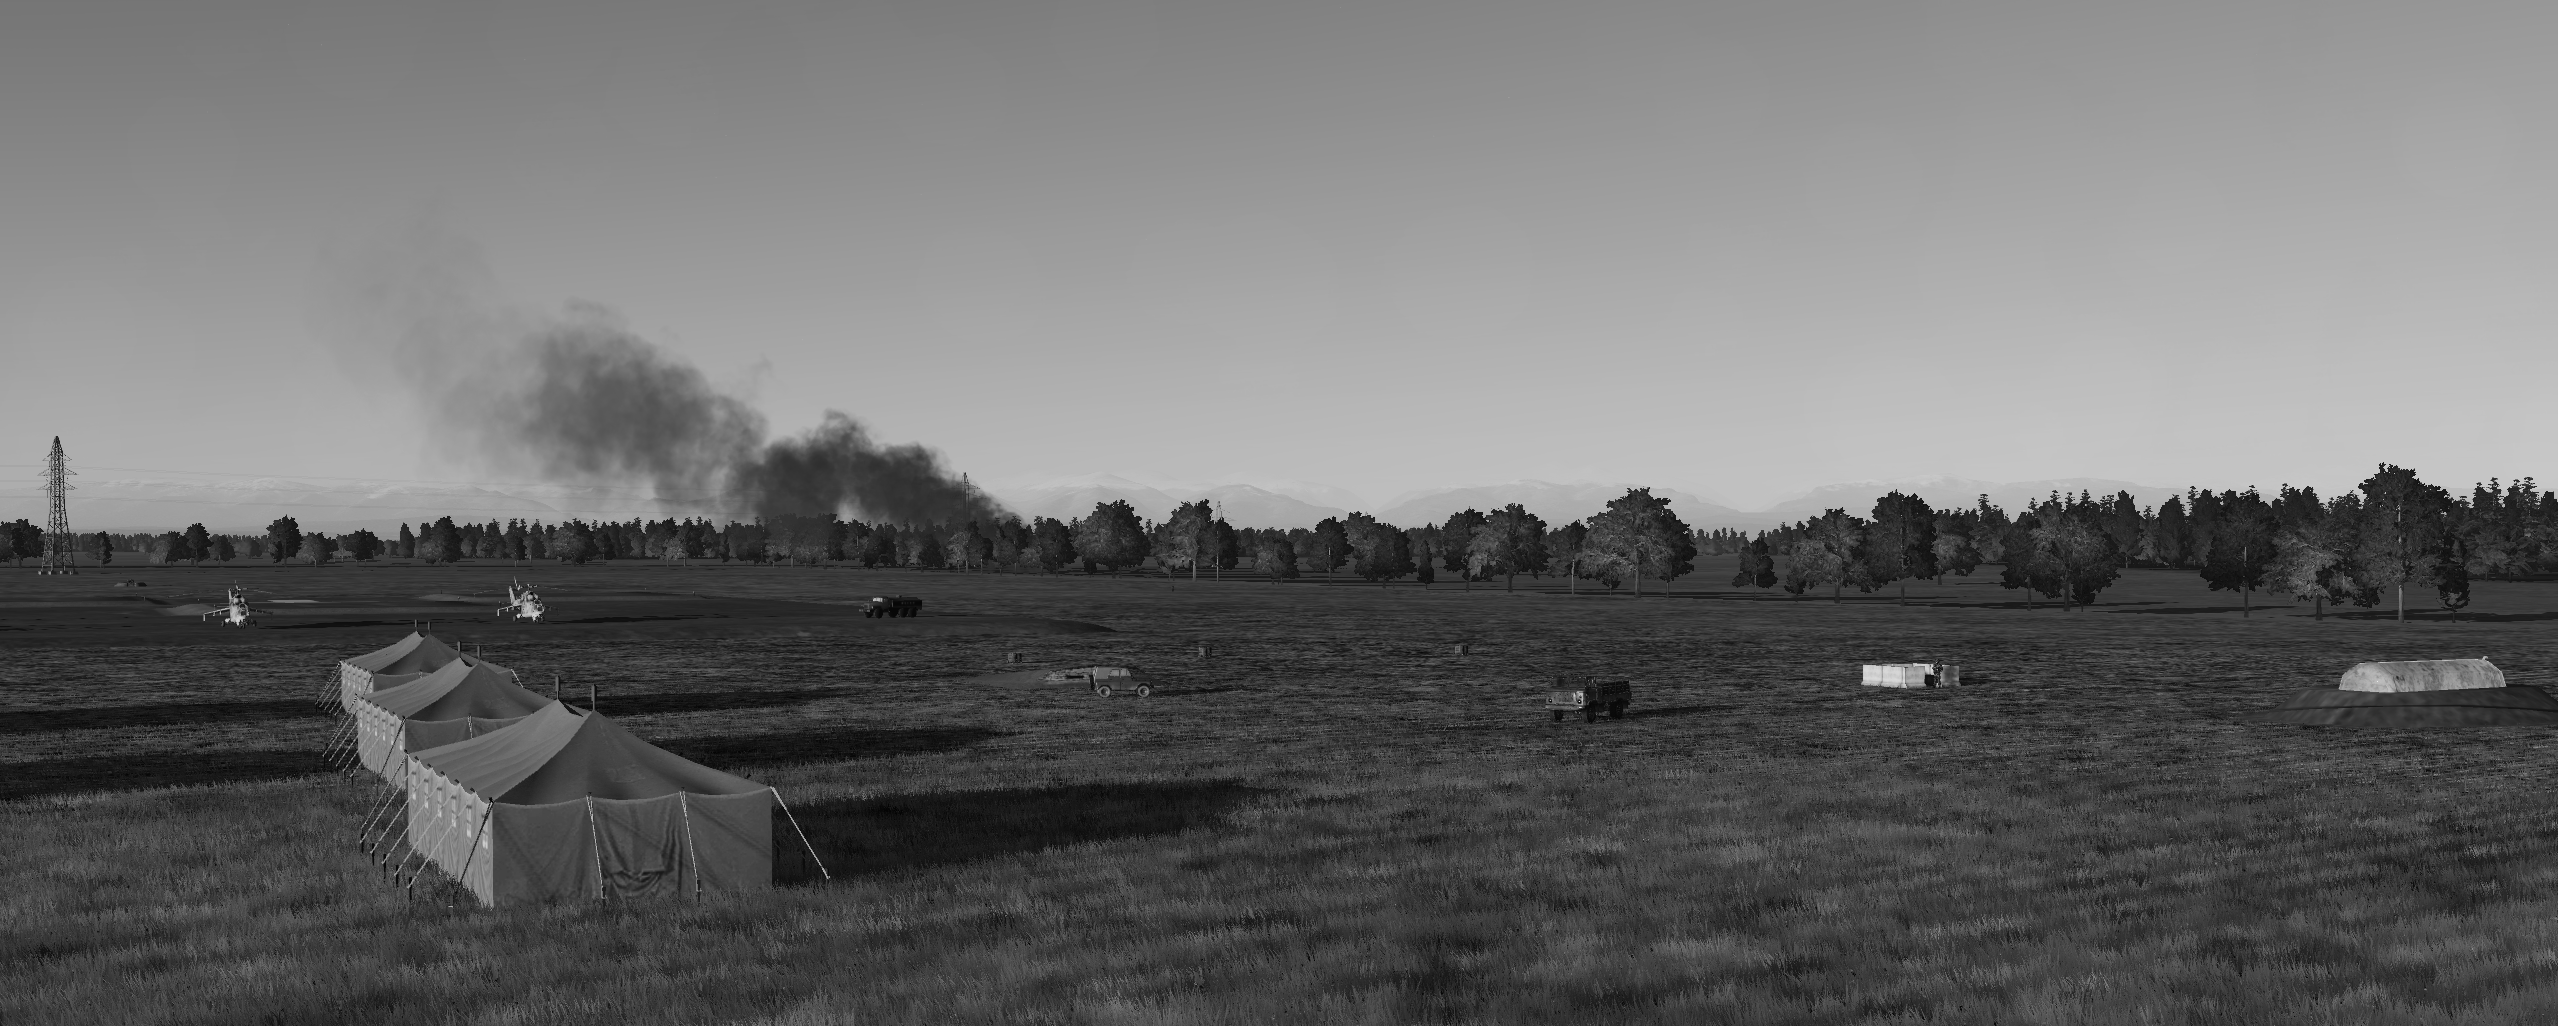
\includegraphics[width=0.7\linewidth]{../gimp/FARP_Skala_Pic.png}
\end{center}
%
% ---------------------------------------------------------------------------------------------------
\newpage
% PRE-FLIGHT
\begin{itemize}
 \item[] \myHead{SEAD Crimea}
 \item[\ri] Threat: SA-10 Grumble
 \item[\ri] Position: N042\,11\;22 E42\,11\,22
\end{itemize}
\begin{center}
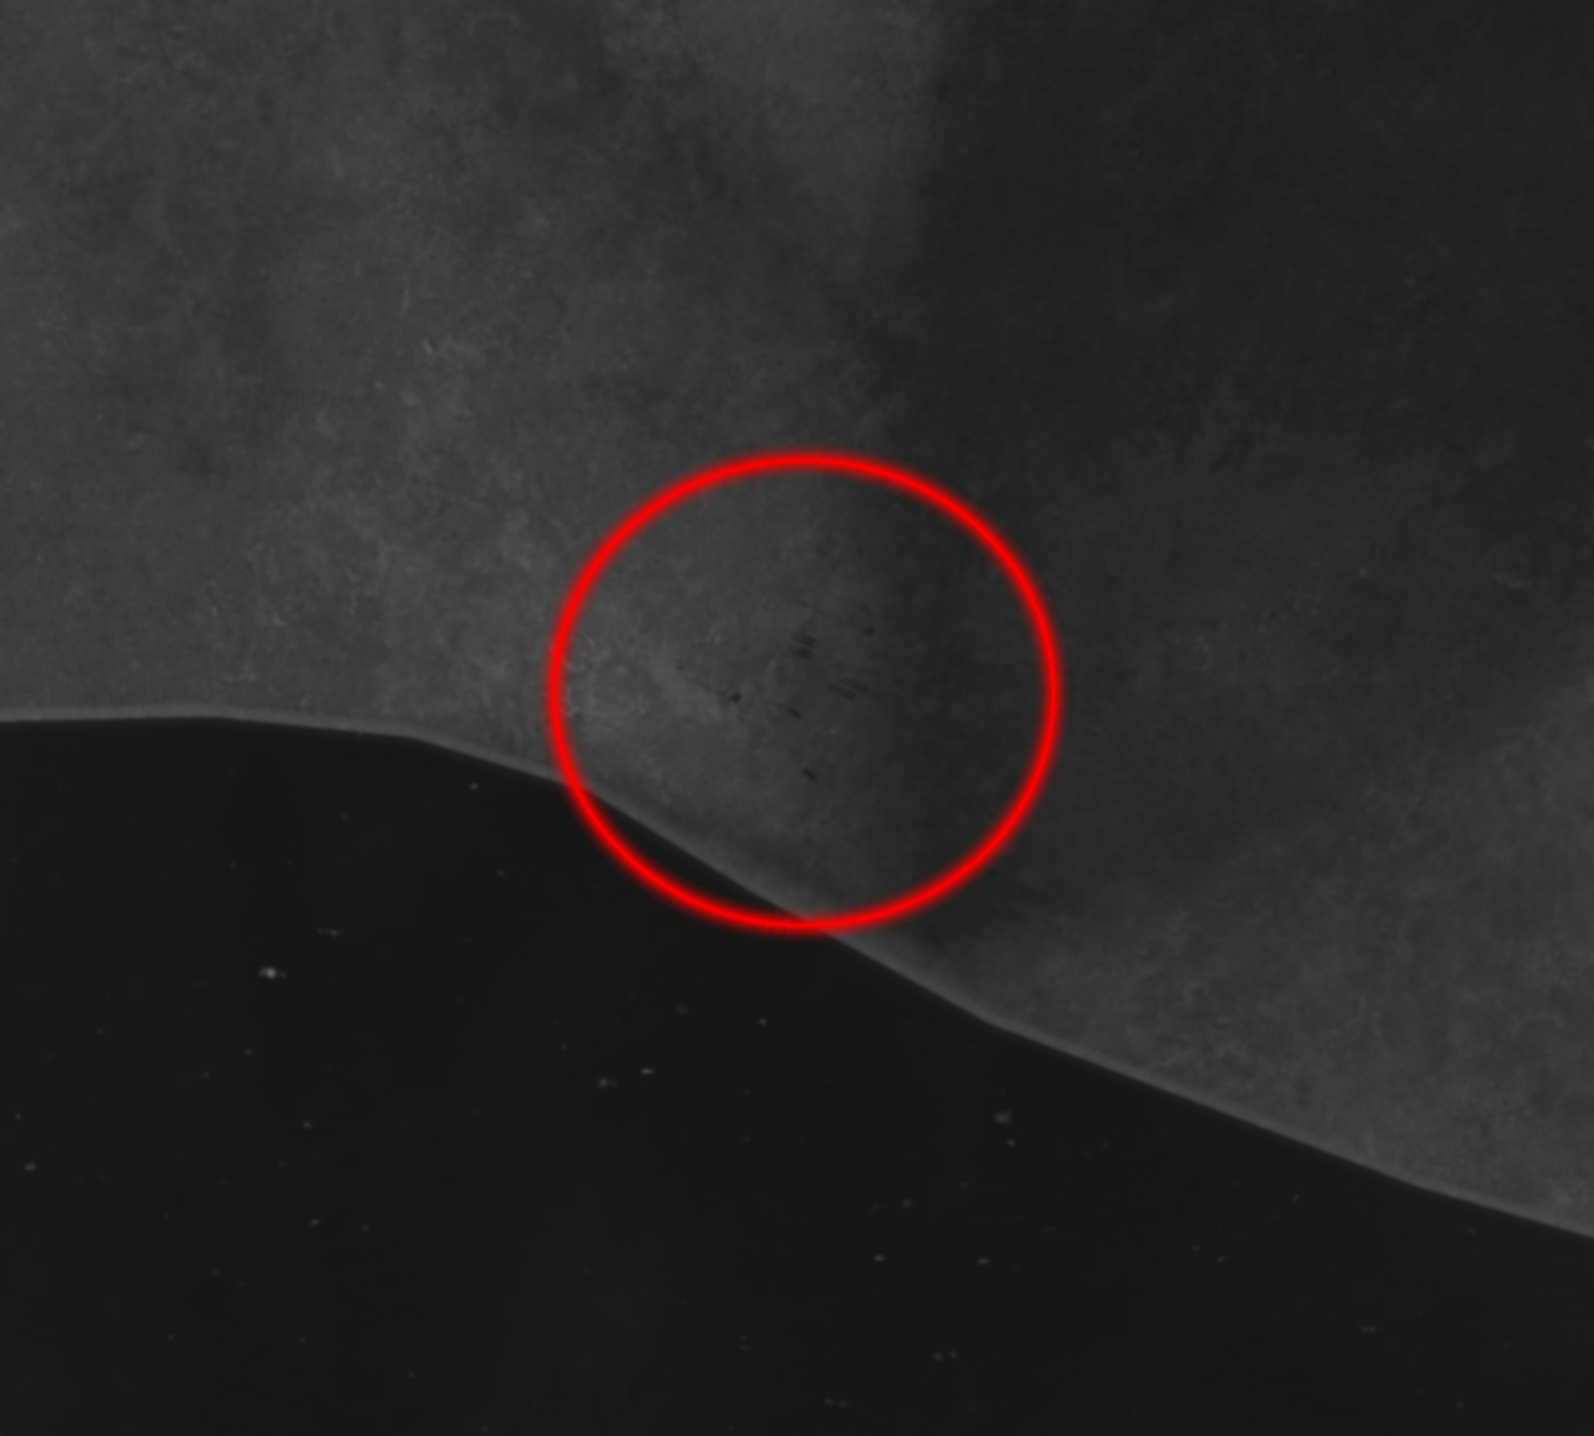
\includegraphics[width=0.7\linewidth]{../gimp/SA10_01.png}
\end{center}
\vspace{1em}
\begin{center}
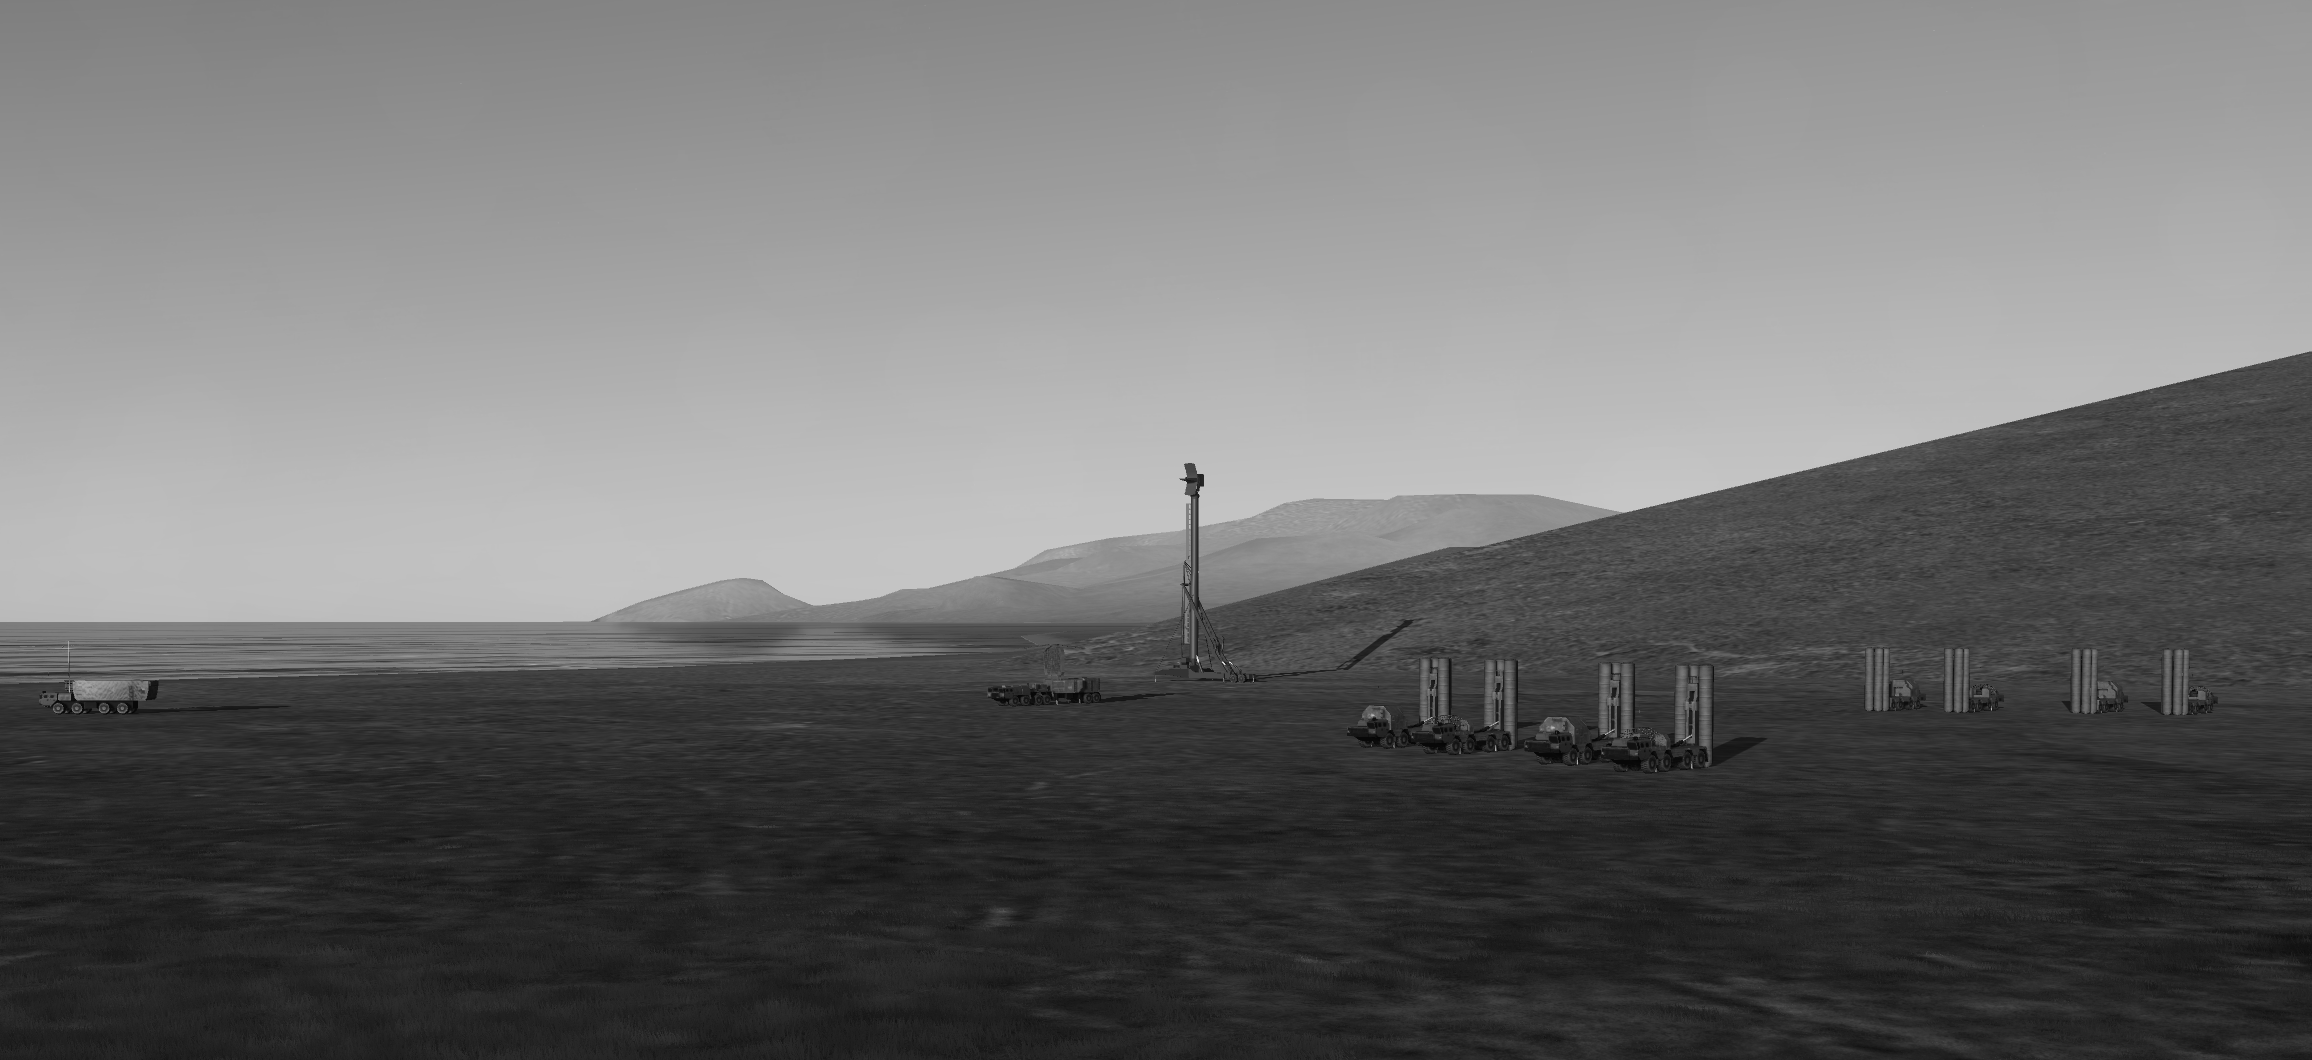
\includegraphics[width=0.7\linewidth]{../gimp/SA10_02.png}
\end{center}
% 
% ---------------------------------------------------------------------------------------------------
\vspace{0.5em}
\newpage
% ENGINE START
\begin{itemize}
 \item[] \myHead{SEAD Maykop}
 \item[\ri] Threat: SA-15 Gauntlet
 \item[\ri] Position: N042\,11\;22 E42\,11\,22 
\end{itemize}
%
\begin{center}
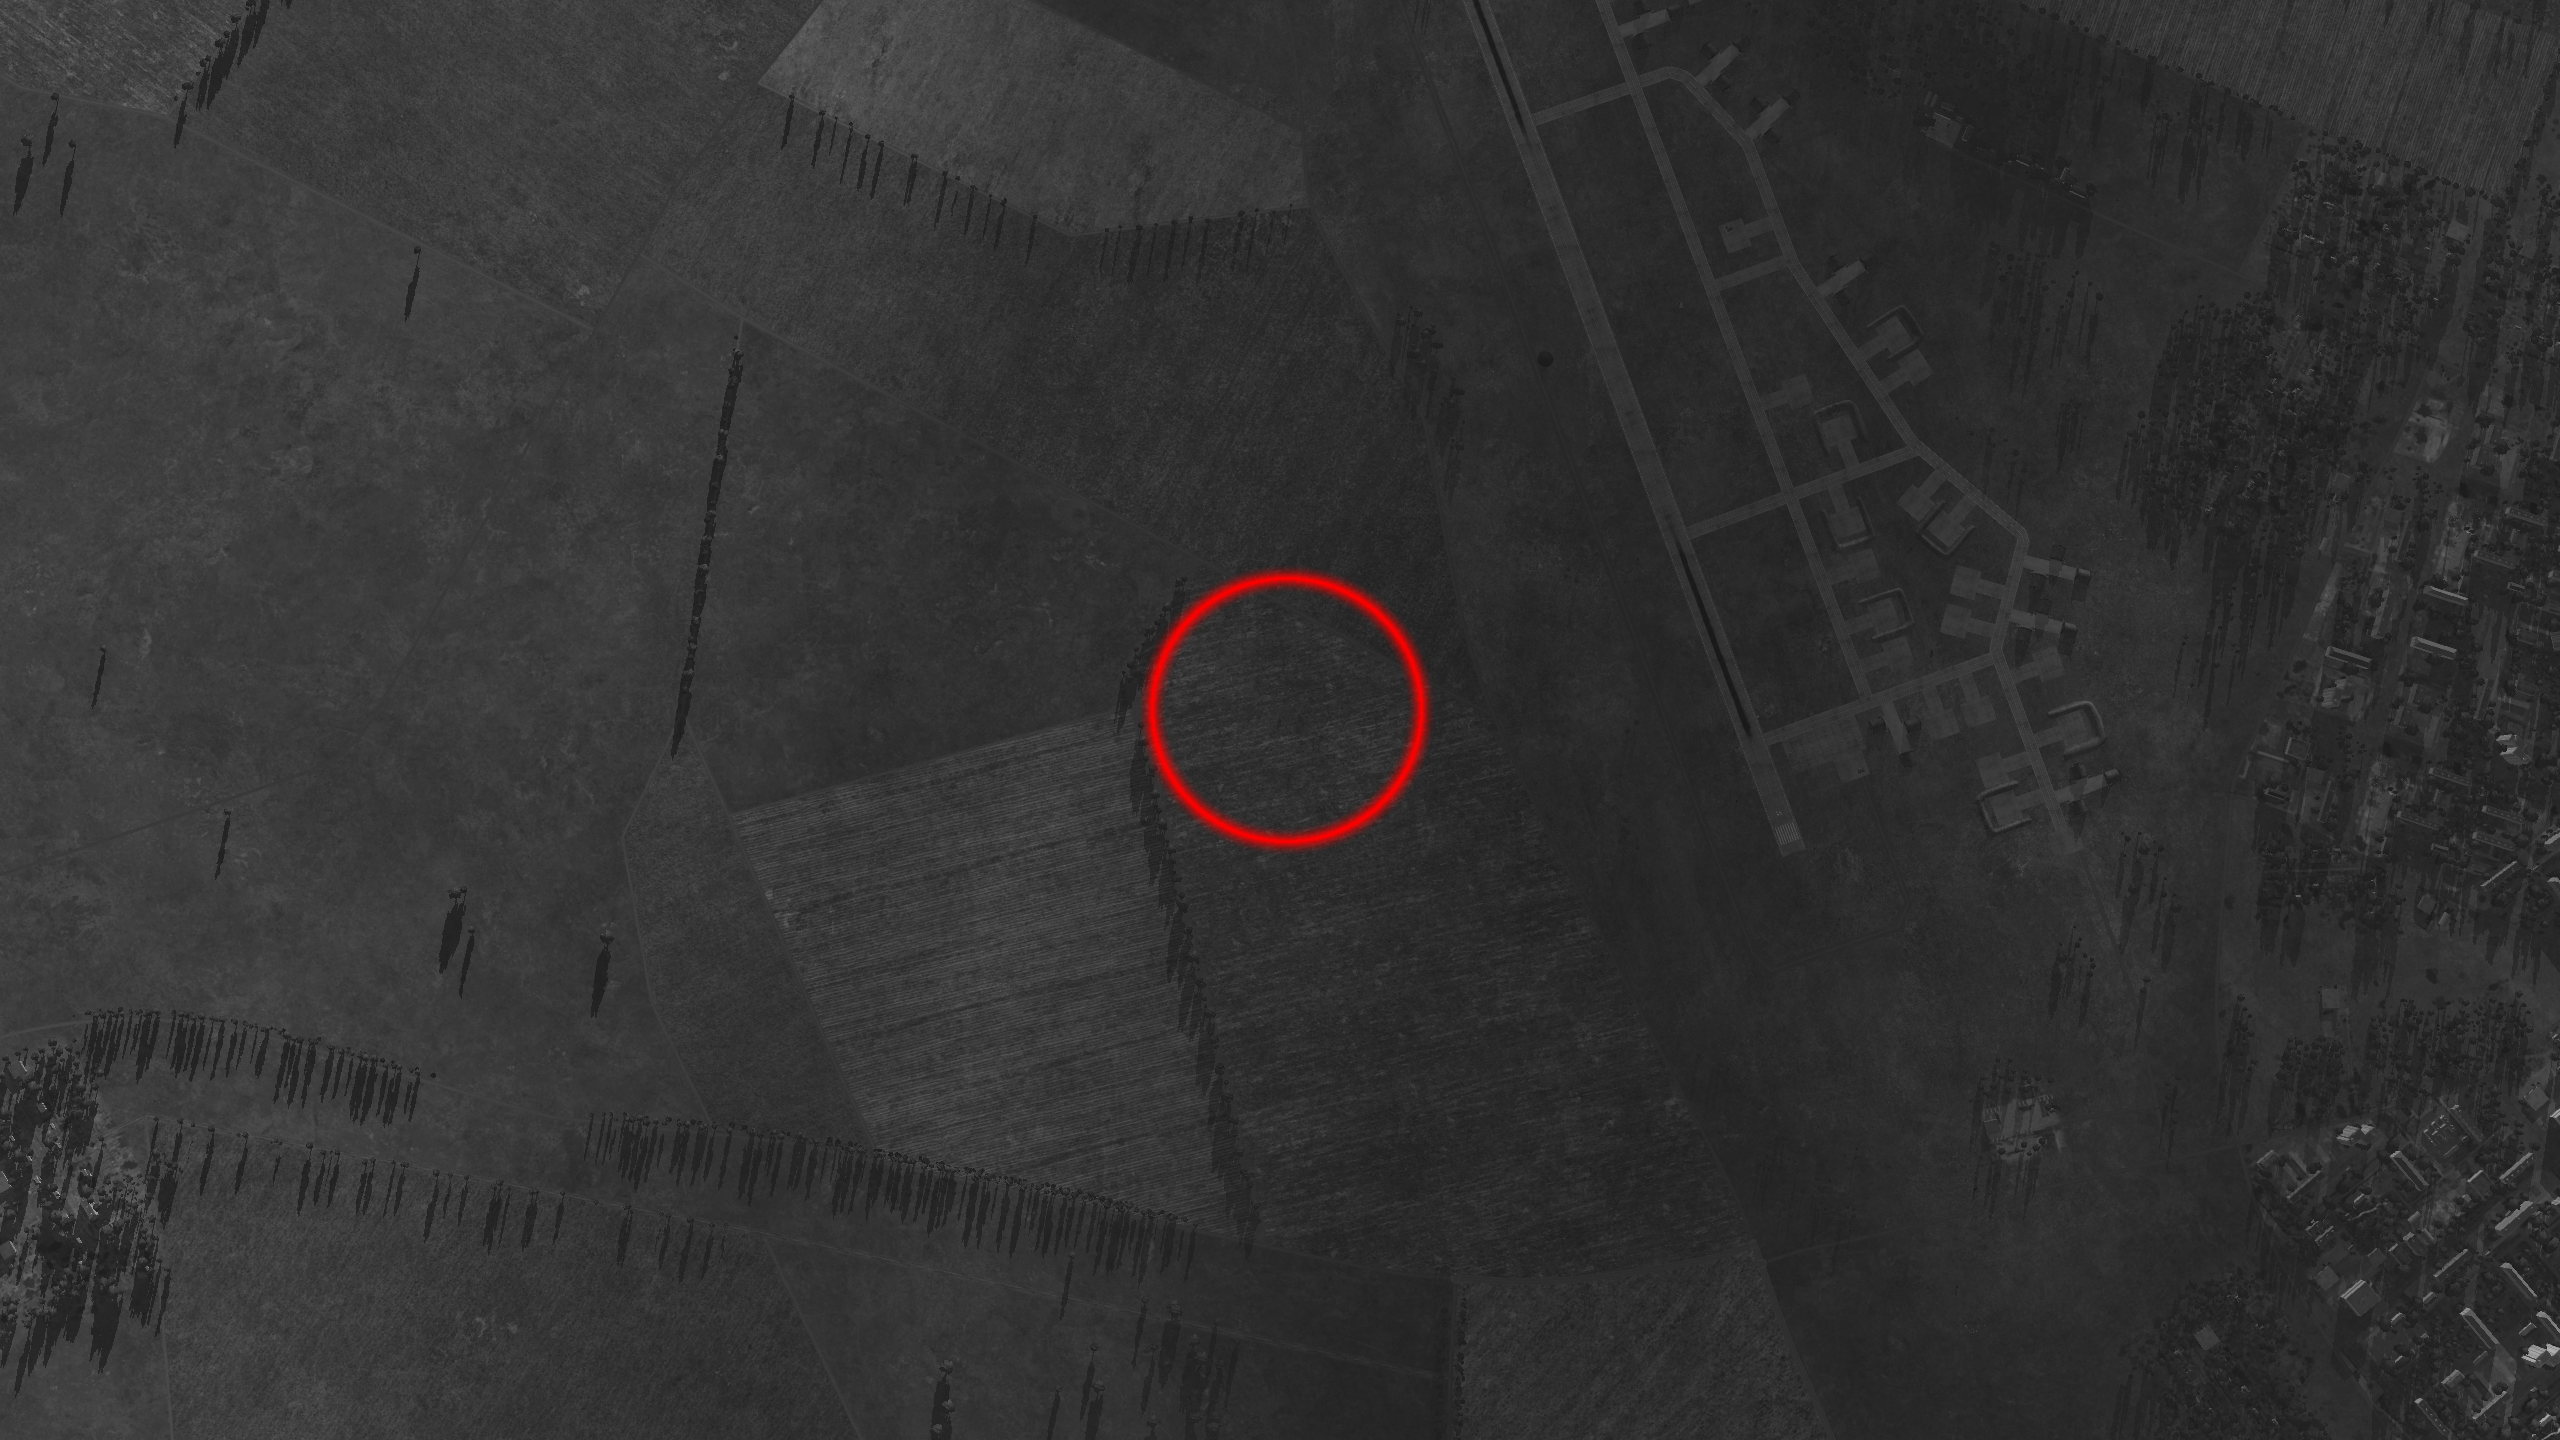
\includegraphics[width=0.7\linewidth]{../gimp/SA15_Sat.png}
\end{center}
%
\begin{itemize}
 \item[\ri] Threat: SA-8 Gecko
 \item[\ri] Position: N042\,11\;22 E42\,11\,22 
\end{itemize}
%
\begin{center}
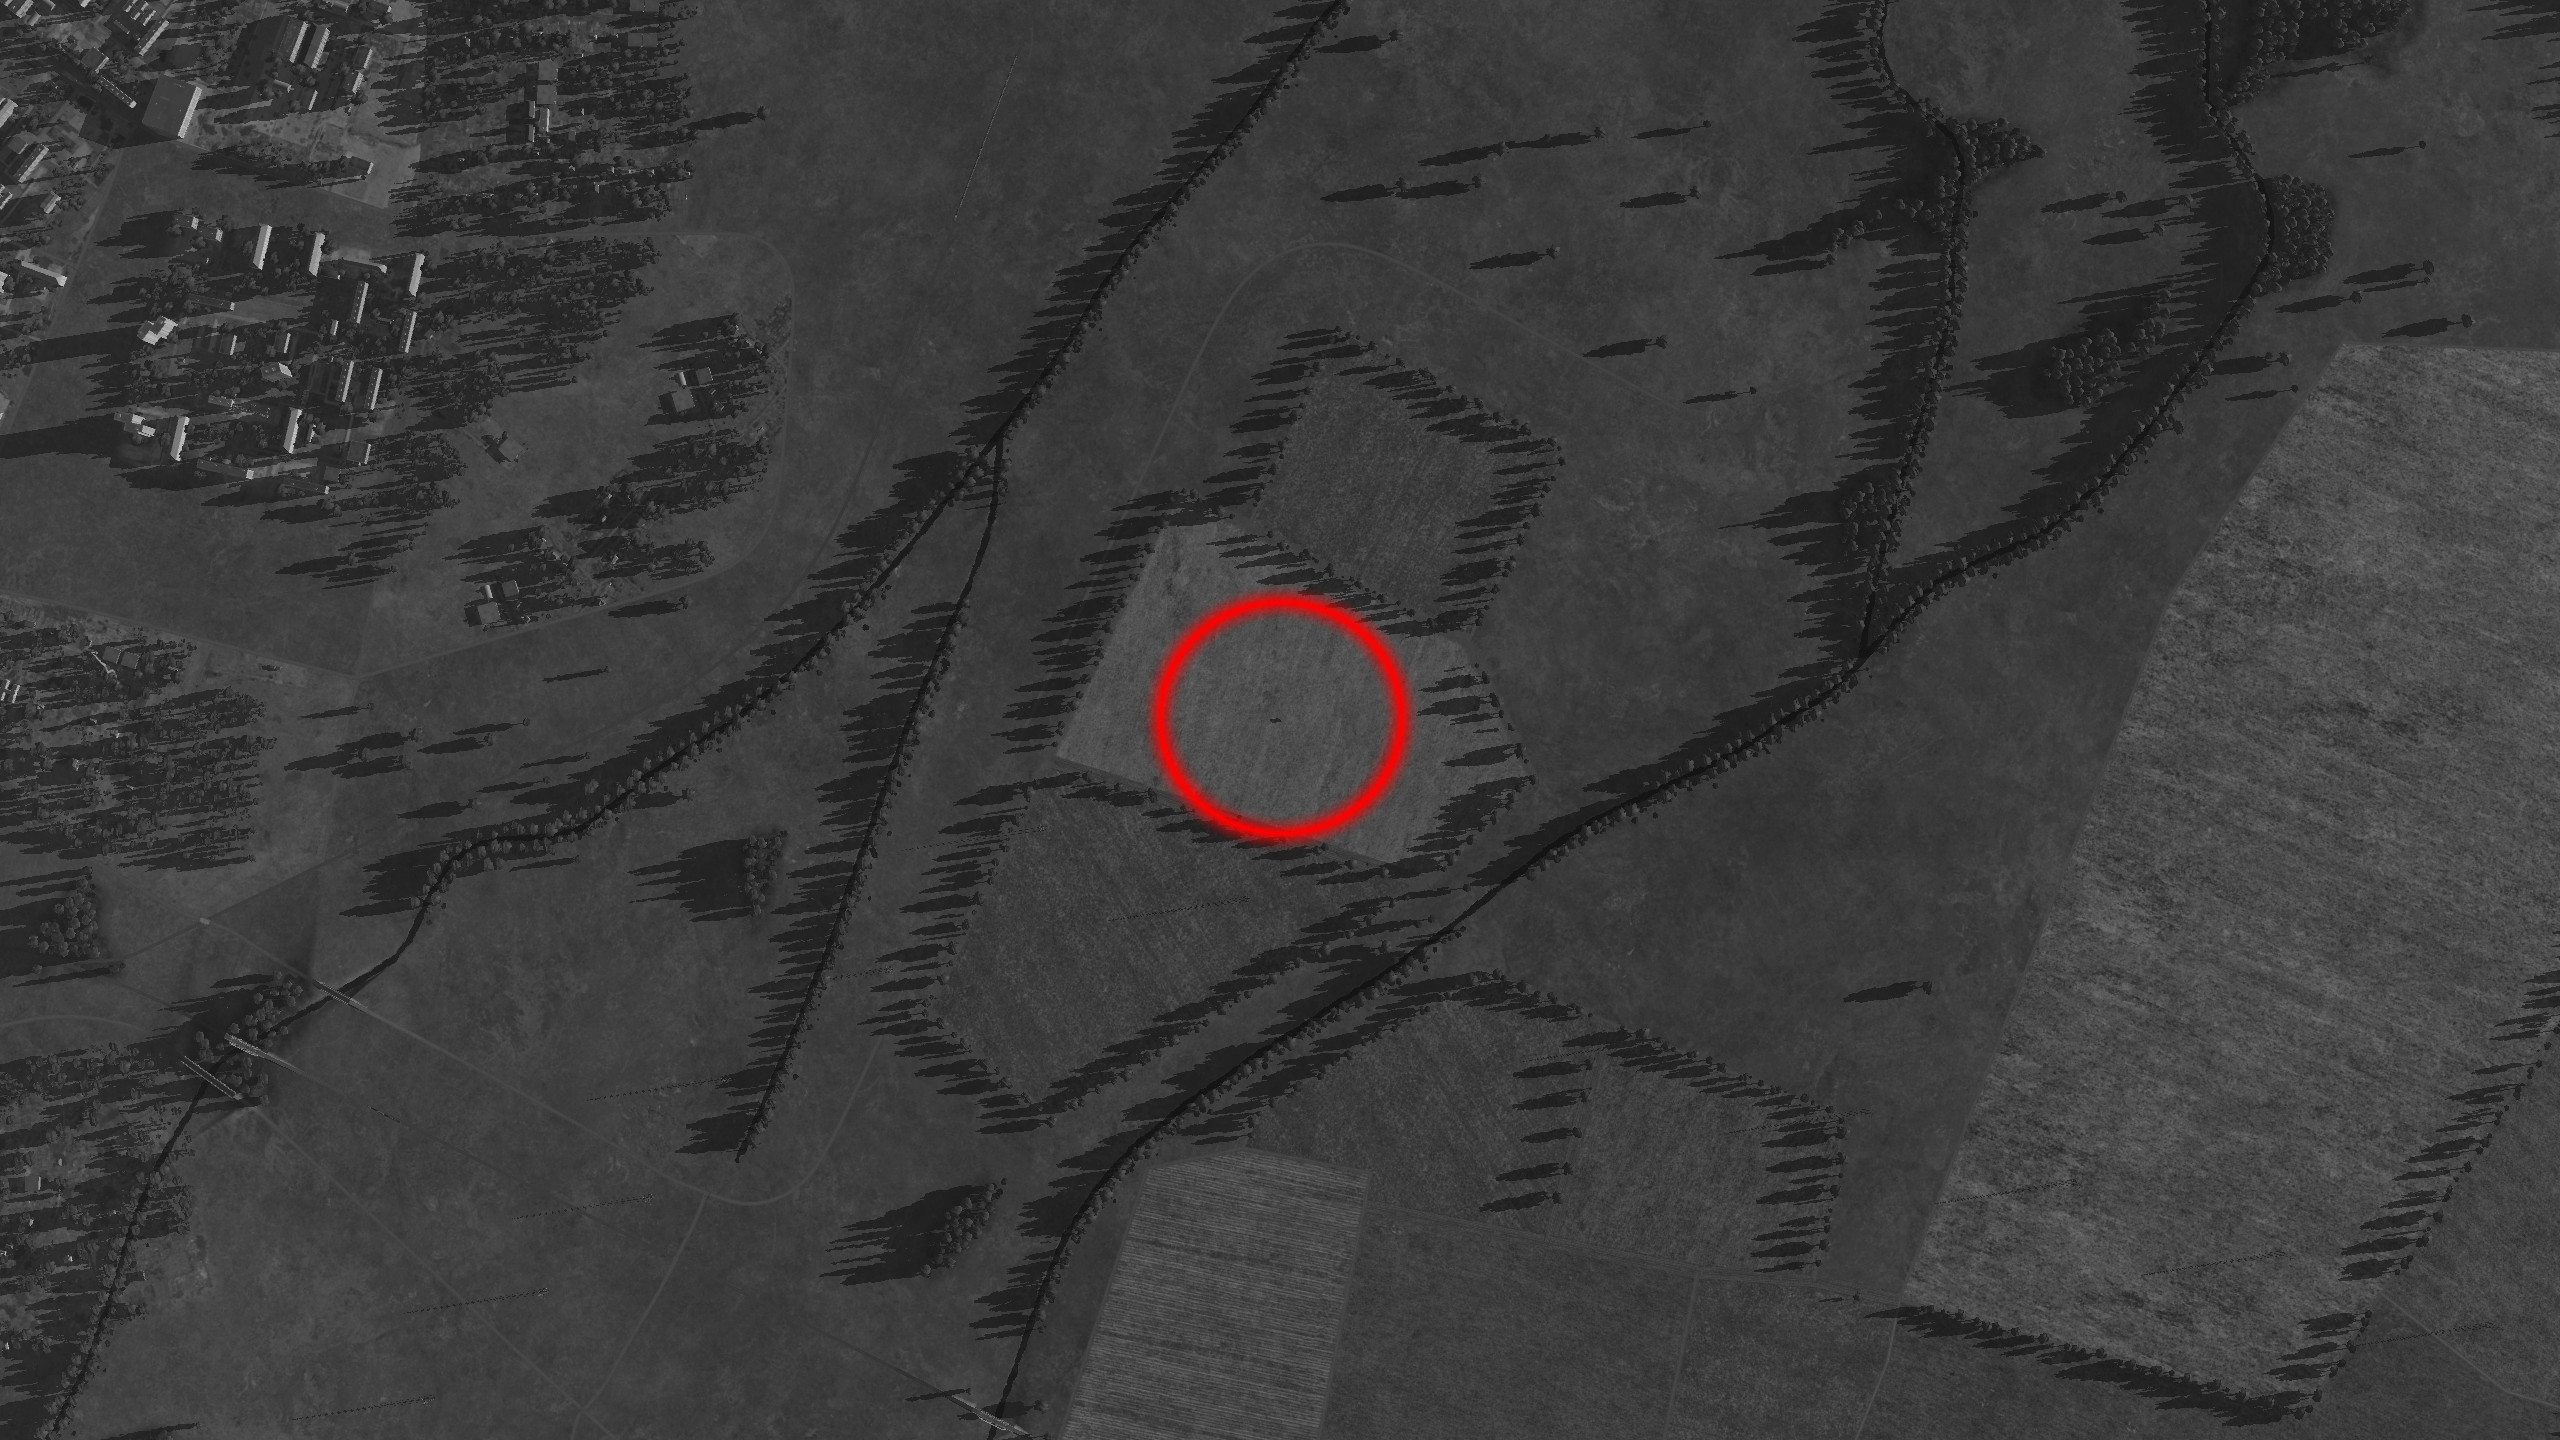
\includegraphics[width=0.7\linewidth]{../gimp/SA8_Sat.png}
\end{center}
%
%
% ---------------------------------------------------------------------------------------------------
% \newpage
% % Field Landing Pattern
% \begin{itemize}
%  \item[] \myHead{Field Landing Pattern}
% \end{itemize}
% % ---------------------------------------------------------------------------------------------------
% \newpage
% % Field Landing Pattern
% \begin{itemize}
%  \item[] \myHead{Carrier Landing Pattern}
% \end{itemize} 
% ---------------------------------------------------------------------------------------------------
%
}
\end{document}
%
